\chapter{Theory of Neutrino Oscillations}
\label{ch:Theory}

The idea of neutrino oscillations was first proposed by Pontecorvo in 1957 \cite{ref:Pontecorvo1}, but his proposal described oscillations between neutrinos and anti-neutrinos. In 1962, after the discovery of the muon neutrino, Maki, Nakagawa, and Sakata proposed the theory that described oscillations between neutrino flavors due to differing neutrino flavor and mass eigenstates \cite{ref:MNS}. This chapter describes the modern formalism in detail and uses natural units where $\hbar = c = 1$, except where otherwise noted.

\section{The PMNS Matrix}
\label{sec:TheoryPMNS}

\begin{figure}[h]
  \begin{center} $
  \begin{array}{c c}
    {
    \begin{fmffile}{Wint}
      \begin{fmfgraph*}(150,150)
        \fmfleft{n1}
        \fmfright{l1}
        \fmfbottom{w1}
        \fmf{fermion}{n1,v1}
        \fmf{fermion}{v1,l1}
        \fmf{photon, tension=.5, label=$W^+$}{v1,w1}
        \fmflabel{$\nu_\ell$}{n1}
        \fmflabel{$\ell^-$}{l1}
      \end{fmfgraph*}
    \end{fmffile}
    }
    \quad \quad & \quad \quad
    {
    \begin{fmffile}{Zint}
      \begin{fmfgraph*}(150,150)
        \fmfleft{n1}
        \fmfright{l1}
        \fmfbottom{w1}
        \fmf{fermion}{n1,v1}
        \fmf{fermion}{v1,l1}
        \fmf{photon, tension=.5, label=$Z^0$}{v1,w1}
        \fmflabel{$\nu_\ell$}{n1}
        \fmflabel{$\nu_\ell$}{l1}
      \end{fmfgraph*}
    \end{fmffile}
    }
  \end{array} $
  \vspace{3 mm}
  \caption[Standard Model Neutrino Interaction Diagrams]{Standard Model Weak interactions involving a neutrino. Left: Charged current interaction. Right: Neutral current interaction.}
  \label{fig:WZ}
  \end{center}
\end{figure}

In the Standard Model, neutrinos only interact via the W and Z bosons as shown by the Feynman diagrams in Fig.~\ref{fig:WZ}. From these diagrams, it is clear that neutrinos always interact in a definite flavor eigenstate, $\ket{\nu_\alpha}$. Furthermore, when a neutrino is produced from a W boson, the flavor is always determined by the associated charged lepton shown in eq.~\ref{eq:NuLepPairs}.
\beq
\begin{pmatrix} \nue \\ e \end{pmatrix}, \quad \begin{pmatrix} \numu \\ \mu \end{pmatrix}, \quad \begin{pmatrix} \nutau \\ \tau \end{pmatrix}
\label{eq:NuLepPairs}
\eeq

\n On the other hand, neutrinos propagate through spacetime with a definite mass, $\ket{\nu_i}$ an eigenstate of the free Hamiltonian. The flavor states can be written as a superposition of the mass states via
\beq
\ket{\nu_\alpha} = \sum_{i=1}^n \Ustxy{\alpha}{i} \ket{\nu_i},
\label{eq:massflav}
\eeq

\n where $n$ is the number of neutrinos, and $U$ is the unitary PMNS matrix, named after Pontecorvo, Maki, Nakagawa, and Sakata. The PMNS matrix is unitary, and would reduce to the identity matrix if neutrinos did not oscillate between flavor states. Yet since it does provide the mechanism for flavor transitions, it can be thought of as analogous to the quark sector CKM matrix.

\section{Vacuum Oscillations}

In this section, the basics of neutrino oscillations are developed by considering oscillations in a vacuum. The neutrinos are treated as plane waves, as in \cite{ref:PlaneWaves}, with the assumption that the neutrino is actually localized in space put in by hand. A careful, rigorous analysis treating the neutrinos as plane waves in \cite{ref:WavePackets} reproduces the same results.

Consider a neutrino in a state of definite flavor $\alpha$ at time $t = 0$, $\ket{\nu(0)} = \ket{\nu_\alpha}$. This state is in a superposition of mass eigenstates. The time evolution of this neutrino is simply the time evolution of the individual mass states. In a vacuum, this adds a phase factor to each mass state.
\beq
\ket{\nu_\alpha(t)} = \sum_{i} \Ustxy{\alpha}{i} e^{-i(E_i t - \mathbf{p_i \cdot x})} \ket{\nu_i}
\label{eq:NuAtT}
\eeq

\n With the neutrino at position $\mathbf{x} = L$ at time $t$, the dot product evaluates to $\mathbf{p_i \cdot x} = p_i L$. Eq~\ref{eq:NuAtT} can then simplified by making use of the fact that neutrinos are ultra-relativistic, allowing for several assumptions. First, the time, $t$, is replaced by the distance, $L$. Next, the energy of each mass state is approximated to be the same energy, $E_i = E$. Last, the momentum is expanded as $p_i = \sqrt{E^2 - m_i^2} \approx E - m_i^2/2E$. With these assumptions, eq.~\ref{eq:NuAtT} simplifies as:
\beq
\ket{\nu_\alpha(L)} = \sum_{i} \Ustxy{\alpha}{i} e^{-i m_i^2 L/2E} \ket{\nu_i}.
\label{eq:NuAtTRel}
\eeq

\n The mass eigenstate inside the sum is then re-expressed in terms of flavor eigenstates using the inverse of eq.~\ref{eq:massflav} and unitarity of $U$.
\beq
\ket{\nu_\alpha(L)} = \sum_{\alpha'} \sum_{i} \Ustxy{\alpha}{i} \Uxy{\alpha'}{i} e^{-i m_i^2 L/2E} \ket{\nu_\alpha'}.
\label{eq:NuAtL}
\eeq

Eq.~\ref{eq:NuAtL} can then be used to find the probability that the original neutrino in flavor state $\alpha$ has transitioned (or survived) as flavor state $\beta$. First, the matrix element $\braket{\nu_\beta | \nu_\alpha (L)}$ is computed.
\beq
\braket{\nu_\beta | \nu_\alpha( L ) } = \sum_{\alpha'} \sum_{i} \Ustxy{\alpha}{i} \Uxy{\alpha'}{i} e^{-i m_i^2 L/2E} \braket{\nu_\beta | \nu_\alpha'}
= \sum_i \Ustxy{\alpha}{i} \Uxy{\beta}{i} e^{-i m_i^2 L/2E}
\label{eq:nuAB}
\eeq

\n The last equality in eq.~\ref{eq:nuAB} follows from the orthogonality of individual flavor eigenstates. The probability of the flavor transition is then the square of this matrix element.
\beq
P(\nu_\alpha \rightarrow \nu_\beta) = \vert \braket{\nu_\beta | \nu_\alpha(L)} \vert^2
= \sum_{i, j} \Ustxy{\alpha}{i} \Uxy{\beta}{i} \Ustxy{\beta}{j} \Uxy{\alpha}{j} e^{-i (m_i^2 - m_j^2) L/2E}
\label{eq:nuABsq}
\eeq

\n It is standard to rewrite the mass squared difference as $\dmxy{j}{i} \equiv m_i^2 - m_j^2$. Eq.~\ref{eq:nuABsq} is then manipulated using the properties of unitary matrices.
\beqa
P(\nu_\alpha \rightarrow \nu_\beta) & = & \sum_{i, j} \Ustxy{\alpha}{i} \Uxy{\beta}{i} \Ustxy{\beta}{j} \Uxy{\alpha}{j} + \sum_{i, j} \Ustxy{\alpha}{i} \Uxy{\beta}{i} \Ustxy{\beta}{j} \Uxy{\alpha}{j} (e^{-i \dmxy{j}{i} L/2E} - 1) \nonumber \\
& = & \delta_{\alpha\beta} + \sum_{i, j} \Ustxy{\alpha}{i} \Uxy{\beta}{i} \Ustxy{\beta}{j} \Uxy{\alpha}{j} (e^{-i \dmxy{j}{i} L/2E} - 1)
\label{eq:nuAB1minus}
\eeqa

\n The remaining summed term is further simplified making use of two facts. When $i = j$, the complex phase is 0 as $\dmxy{i}{i} = 0$, and thus these terms vanish. Second, the terms with $i < j$ are complex conjugates of those with $i > j$, and $z + z^* = 2\Re(z)$ for any complex number $z$.
\beqa
P(\nu_\alpha \rightarrow \nu_\beta) & = & \delta_{\alpha\beta} + 2\sum_{i > j} \Re \left[ \Ustxy{\alpha}{i} \Uxy{\beta}{i} \Ustxy{\beta}{j} \Uxy{\alpha}{j} (e^{-i \dmxy{j}{i} L/2E} - 1) \right]
\label{eq:nuABiGrj}
\eeqa

\n Both pieces of this term are split into their real and imaginary parts, and simplified using the trigonometric identity $\cos2\theta - 1 = -2\sin^2\theta$. Defining\hspace{0.5em}$\mathcal{U} \equiv \Ustxy{\alpha}{i} \Uxy{\beta}{i} \Ustxy{\beta}{j} \Uxy{\alpha}{j} (e^{-i \dmxy{j}{i} L/2E} - 1)$ and $\phi \equiv \dmxy{j}{i} L/2E$:
\beqa
\Re ( \mathcal{U} ) & = & \Re \left[ \Ustxy{\alpha}{i} \Uxy{\beta}{i} \Ustxy{\beta}{j} \Uxy{\alpha}{j} (e^{-i \dmxy{j}{i} L/2E} - 1) \right] \\
%& = & \Re \left\{ \left[ \Re ( \Ustxy{\alpha}{i} \Uxy{\beta}{i} \Ustxy{\beta}{j} \Uxy{\alpha}{j} ) + i \Im ( \Ustxy{\alpha}{i} \Uxy{\beta}{i} \Ustxy{\beta}{j} \Uxy{\alpha}{j} ) \right] \left[ \cos\phi - i\sin\phi - 1\right] \right\} \\
& = & \Re \left\{ \left[ \Re ( \Ustxy{\alpha}{i} \Uxy{\beta}{i} \Ustxy{\beta}{j} \Uxy{\alpha}{j} ) + i \Im ( \Ustxy{\alpha}{i} \Uxy{\beta}{i} \Ustxy{\beta}{j} \Uxy{\alpha}{j} ) \right] \left[ -2\sin^2 (\phi/2) - i\sin\phi \right] \right\} \\
%& = & \Re \left\{ -2 \Re ( \Ustxy{\alpha}{i} \Uxy{\beta}{i} \Ustxy{\beta}{j} \Uxy{\alpha}{j} ) \sin^2 (\phi/2) + \Im ( \Ustxy{\alpha}{i} \Uxy{\beta}{i} \Ustxy{\beta}{j} \Uxy{\alpha}{j} ) \sin\phi \right. \nonumber \\
%&& \quad\quad \left. -i \left[ \Re ( \Ustxy{\alpha}{i} \Uxy{\beta}{i} \Ustxy{\beta}{j} \Uxy{\alpha}{j} ) \sin\phi + 2\Im ( \Ustxy{\alpha}{i} \Uxy{\beta}{i} \Ustxy{\beta}{j} \Uxy{\alpha}{j} ) \sin^2 (\phi/2) \right] \right\} \\
& = & -2 \Re ( \Ustxy{\alpha}{i} \Uxy{\beta}{i} \Ustxy{\beta}{j} \Uxy{\alpha}{j} ) \sin^2 (\phi/2) + \Im ( \Ustxy{\alpha}{i} \Uxy{\beta}{i} \Ustxy{\beta}{j} \Uxy{\alpha}{j} ) \sin\phi
\label{eq:ExpandUUUUe1}
\eeqa

\n Inserting the expression from eq.~\ref{eq:ExpandUUUUe1} into eq.~\ref{eq:nuABiGrj}, we find:
\beqa
P(\nu_\alpha \rightarrow \nu_\beta) = \delta_{\alpha\beta} & - & 4\sum_{i > j} \Re ( \Ustxy{\alpha}{i} \Uxy{\beta}{i} \Ustxy{\beta}{j} \Uxy{\alpha}{j} ) \sin^2 \left( \frac{\dmxy{j}{i} L}{4E} \right) \nonumber \\
& + & 2\sum_{i > j} \Im ( \Ustxy{\alpha}{i} \Uxy{\beta}{i} \Ustxy{\beta}{j} \Uxy{\alpha}{j} ) \sin \left( \frac{\dmxy{j}{i} L}{2E} \right),
\label{eq:nuOsc}
\eeqa

\n which is the standard equation for neutrino oscillations. It can now be seen that the distance the neutrino travels, its energy, and the different mass splittings all affect the frequency of oscillation. Ideally, neutrino oscillations would be studied by having neutrinos with a fixed energy profile (preferably monoenergetic) and varying the baseline. However, neutrino detectors are incredibly large, so in practice the baseline is fixed and the oscillation probability is studied as a function of neutrino energy. 

For the case of survival probability, $\alpha = \beta$ and eq.~\ref{eq:nuOsc} simplifies further. The imaginary piece from eq.~\ref{eq:nuOsc} drops out, as
\beq
\Im ( \Ustxy{\alpha}{i} \Uxy{\alpha}{i} \Ustxy{\alpha}{j} \Uxy{\alpha}{j} ) = \Im ( \Usqxy{\alpha}{i} \Usqxy{\alpha}{j} ) = 0.
\label{eq:survIm}
\eeq

\n The survival probability is then given by:
\beq
P(\nu_\alpha \rightarrow \nu_\alpha) = 1 - 4 \sum_{i > j} \Usqxy{\alpha}{i} \Usqxy{\alpha}{j} \sin^2 \left( \frac{\dmxy{j}{i} L}{4E} \right).
\label{eq:nuSurv}
\eeq

Due to the combined influence of mass splitting, oscillation baseline, and neutrino energy on the oscillation probability, it is often the case that only one term contributes to the sums in eq.s~\ref{eq:nuOsc} and \ref{eq:nuSurv}. The two neutrino approximation can be instructive in this instance. For this model, the mixing matrix simplifies to the two dimensional rotation matrix:
\beq
U = \begin{pmatrix} \cos\theta & \sin\theta \\ -\sin\theta & \cos\theta \end{pmatrix}.
\label{eq:2NuU}
\eeq

\n As this matrix is entirely real, the imaginary piece of eq.~\ref{eq:nuOsc} drops out. Plugging the matrix elements into the remaining term directly and simplifying slightly, we find the following forms for the survival and appearance probabilities.
\beqa
P(\nu_\alpha \rightarrow \nu_\alpha) & = & 1 - \sin^2 2\theta \sin^2 \left( \frac{\Delta m^2 L}{4E} \right) \label{eq:2NuSurv} \\
P(\nu_\alpha \nrightarrow \nu_\alpha) & = & \sin^2 2\theta \sin^2 \left( \frac{\Delta m^2 L}{4E} \right) \label{eq:2NuApp}
\eeqa

\n From these equations it is clear that the mixing matrix parameters control the amplitude of neutrino oscillations. For small angles, most neutrinos will not change flavor, while larger angles can cause most of the neutrinos to change flavor. The case where $\theta = 45^\circ$ is called maximal mixing as at specific baseline lengths the probability of oscillation becomes 1.

\section{Standard 3-Flavor Oscillations}
\label{sec:Theory3}

The Standard Model includes three neutrinos, so the PMNS matrix is $3 \times 3$ in this picture. Explicitly expanding eq.~\ref{eq:massflav}, $U$ takes the following form:
\beq
\begin{pmatrix} \nue \\ \numu \\ \nutau \end{pmatrix} = \begin{pmatrix} \Uxy{e}{1} & \Uxy{e}{2} & \Uxy{e}{3} \\ \Uxy{\mu}{1} & \Uxy{\mu}{2} & \Uxy{\mu}{3} \\ \Uxy{\tau}{1} & \Uxy{\tau}{2} & \Uxy{\tau}{3} \end{pmatrix} \begin{pmatrix} \nu_1 \\ \nu_2 \\ \nu_3 \end{pmatrix}.
\label{eq:FlavUMass}
\eeq

\n The PMNS matrix can be parametrized in terms of 3 real mixing angles, $\theta_{ij}$ and a complex phase, $\delta$, called the CP phase. Following the convention from the Particle Data Group \cite{ref:PDG}, the expanded matrix takes the form
\beqa
U & = & \begin{bmatrix} c_{12} c_{13} & s_{12} c_{13} & s_{13} e^{-i\delta} \\ -s_{12} c_{23} - c_{12} s_{23} s_{13} e^{i\delta} & c_{12} c_{23} - s_{12} s_{23} s_{13} e^{i\delta} & s_{23} c_{13} \\ s_{12} s_{23} - c_{12} c_{23} s_{13} s^{i\delta} & -c_{12} s_{23} - s_{12} c_{23} s_{13} e^{i\delta} & c_{23} c_{13} \end{bmatrix} \nonumber \\
& = & \begin{bmatrix} 1 & 0 & 0 \\ 0 & c_{23} & s_{23} \\ 0 & -s_{23} & c_{23} \end{bmatrix} \begin{bmatrix} c_{13} & 0 & s_{13} e^{-i\delta} \\ 0 & 1 & 0 \\ -s_{13} e^{i\delta} & 0 & c_{13} \end{bmatrix} \begin{bmatrix} c_{12} & s_{12} & 0 \\ -s_{12} & c_{12} & 0 \\ 0 & 0 & 1 \end{bmatrix}
\label{eq:3NuU}
\eeqa

\n where $c_{ij} \equiv \cos\theta_{ij}$ and $s_{ij} \equiv \sin\theta_{ij}$.

With three neutrinos, the expanded forms of eq.s \ref{eq:nuOsc} and \ref{eq:nuSurv} can still balloon into unwieldy messes. Fortunately, based on current knowledge of the mass splittings, it is usually the case that only one mass splitting scale matters and other terms can be dropped. Fig.~\ref{fig:MassSplit} shows a schematic of the mass splittings. For historic reasons, $\dmxy{1}{2}$ is known as the solar mass splitting and the larger mass splitting is called the atmospheric mass splitting. The atmospheric mass splitting is about 30 times the solar mass splitting. The sign of the solar mass splitting is known, while that of the atmospheric mass splitting is not. A positive value of $\dmxy{2}{3}$ is called the normal hierarchy; a negative value is called the inverted hierarchy.

\begin{figure}[h]
  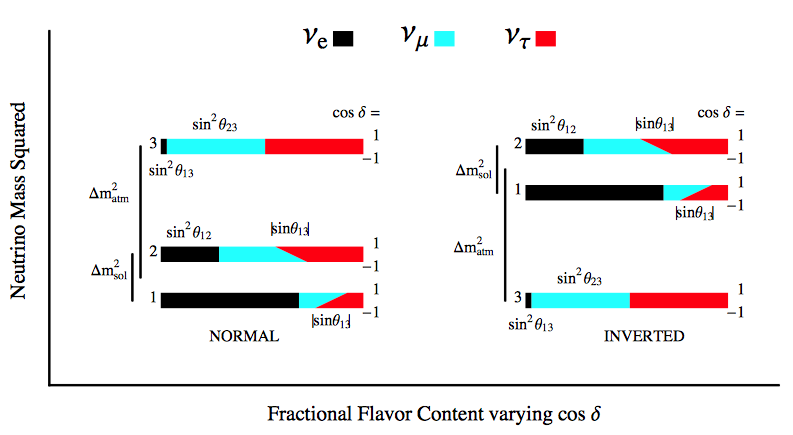
\includegraphics[width=\textwidth]{figures/MassSplitting.png}
  \caption[Neutrino Mass Splitting Schematic]{A schematic of the mass splittings between the three known neutrino mass states and how much they couple to each of the flavor states \cite{ref:MassSplitRef}.}
  \label{fig:MassSplit}
\end{figure}

Two oscillation probabilities that are of interest to \nova~are the muon neutrino survival probability and electron neutrino appearance from a muon neutrino beam. Since $\vert\dmxy{1}{2}\vert$ is so much smaller than $\vert\dmxy{2}{3}\vert$, the solar oscillation baseline is much longer, thus the oscillation probability is first dominated by terms containing $\dmxy{2}{3}$. This is the case for \nova. Furthermore, the probability can be simplified by making making the assumption that $\vert \dmxy{2}{3} \vert \approx \vert \dmxy{1}{3} \vert$. Under these conditions, the survival probability of muon neutrinos is calculated as follows:
\beqa
P(\numu \rightarrow \numu) & \approx & 1 - 4\Usqxy{\mu}{3} (\Usqxy{\mu}{1} + \Usqxy{\mu}{2}) \sin^2 \frac{\dmxy{2}{3} L}{4E} \label{eq:3MuToMu1} \\
& \approx & 1 - 4 s^2_{23} (1 - s^2_{13}) (c^2_{23} + s^2_{23} s^2_{13}) \sin^2 \frac{\dmxy{2}{3} L}{4E} \label{eq:3MuToMu2} \\
& \approx & 1 - 4 s^2_{23} c^2_{23} \sin^2 \frac{\dmxy{2}{3} L}{4E} + 4 s^2_{23} s^2_{13} (c^2_{23} - s^2_{23}) \sin^2 \frac{\dmxy{2}{3} L}{4E} \label{eq:3MuToMu3} \\
& = & 1 - \sin^2 2\thxy{2}{3} \sin^2 \frac{\dmxy{2}{3} L}{4E} + 4 \sin^2 \thxy{2}{3} \sin^2 \thxy{1}{3} \cos^2 2\thxy{2}{3} \sin^2 \frac{\dmxy{2}{3} L}{4E} \quad\quad
\label{eq:3MuToMu}
\eeqa

\n Between eq.s \ref{eq:3MuToMu2} and \ref{eq:3MuToMu3}, the term proportional to $s^4_{13}$ was dropped using the current knowledge that $s^2_{13}$ is small \cite{ref:PDG}. Note that if $\theta_{13}$ were 0, then eq.~\ref{eq:3MuToMu} would reduce to eq.~\ref{eq:2NuSurv}, the two neutrino survival probability.

The full 3 flavor electron neutrino appearance from muon neutrino oscillation probability is often written in the form \cite{ref:Evan}:
\beq
P(\nuanu_{\mu} \rightarrow\,\nuanu_{e}) = P_{atm} + 2\sqrt{P_{atm}}\sqrt{P_{sol}} \left(\cos\delta \cos\frac{\dmxy{2}{3}L}{4E}\, \varmp\, \sin\delta \sin\frac{\dmxy{2}{3}L}{4E} \right) + P_{sol}
\label{eq:3MuToE}
\eeq

\n where
\beqa
\sqrt{P_{atm}} & \equiv & \sin \thxy{2}{3} \sin 2\thxy{1}{3} \sin \frac{\dmxy{2}{3} L}{4E} \label{eq:Patm} \\
\sqrt{P_{sol}} & \equiv & \cos \thxy{2}{3} \sin 2\thxy{1}{2} \sin \frac{\dmxy{1}{2} L}{4E} \label{eq:Psol}
\eeqa

\n where the approximation $\vert \dmxy{2}{3} \vert \approx \vert \dmxy{1}{3} \vert$ has been made and higher order terms of $s^2_{13}$ been dropped. For an experiment at a short enough baseline such as \nova, the $P_{sol}$ term is negligible as it depends on a higher order term of the solar mass splitting. The cross term is also not the dominant effect as it also depends upon the solar mass splitting, but it demonstrates interesting behavior. The $\cos\delta$ term is $CP$ conserving, but the $\sin\delta$ term exhibits $CP$ violation. This is why $\delta$ is called the $CP$ violating phase angle.

\section{Matter Effects}
\label{sec:TheoryMatter}

So far, the oscillation formalism has been developed only considering neutrinos in a vacuum. However, most neutrino oscillation experiments involve neutrinos traveling through matter, be it the Sun or the Earth. This affects the oscillation probabilities in a process called the Mikheyev-Smirnov-Wolfenstein effect, or MSW effect. The phenomenon was first proposed by Wolfenstein in 1978 \cite{ref:Wolfenstein}; Mikheyev and Smirnov built upon that work in 1985 \cite{ref:MSW} as a possible solution for the solar neutrino problem.

\begin{figure}[t]
  \begin{center} $
  \begin{array}{c c}
    {
    \begin{fmffile}{MSWnue}
      \begin{fmfgraph*}(150,120)
        \fmfleft{n1,l2}
        \fmfright{l1,n2}
        \fmf{fermion}{n1,v1,l1}
        \fmf{fermion}{l2,v2,n2}
        \fmf{photon, tension=.75, label=$W^-$}{v1,v2}
        \fmflabel{$\nue$}{n1}
        \fmflabel{$e$}{l1}
        \fmflabel{$\nue$}{n2}
        \fmflabel{$e$}{l2}
      \end{fmfgraph*}
    \end{fmffile}
    }
    \quad \quad & \quad \quad
    {
    \begin{fmffile}{MSWanue}
      \begin{fmfgraph*}(150,120)
        \fmfleft{n1,l1}
        \fmfright{n2,l2}
        \fmf{fermion}{l1,v1,n1}
        \fmf{fermion}{n2,v2,l2}
        \fmf{photon, tension=.75, label=$W^-$}{v1,v2}
        \fmflabel{$\nue$}{n1}
        \fmflabel{$e$}{l1}
        \fmflabel{$\nue$}{n2}
        \fmflabel{$e$}{l2}
      \end{fmfgraph*}
    \end{fmffile}
    }
  \end{array} $
  \vspace{3 mm}
  \caption[MSW Effect Interactions]{Coherent forward scattering interactions involved in the MSW effect. Left: Scattering of electron neutrinos on electrons. Right: Scattering of anti-electron neutrinos on electrons.}
  \label{fig:MSW}
  \end{center}
\end{figure}

The MSW effect is the coherent forward scattering of neutrinos off of the electrons in ordinary matter, a channel only available to electron flavor neutrinos and anti-neutrinos. Fig.~\ref{fig:MSW} illustrates the interactions.

\subsection{Current Measurements}
\label{sec:BestMeasures}

\section{Sterile Neutrinos}
\label{sec:Theory3+1}

\section{Neutrino Mass in the Standard Model}
